\chapter{Latency, fidelity and congestion across memory budgets (Experiment 1)}
\label{ch:exp1}

\section{Design}
All ten benchmarks, on the corrected scheduler, with $1,2,3,4,6,8,16,32$ communication memories per core (QFT also $64$). Budgets $1$--$4$ are \emph{modelled}
(the group's multi-core paper gives four communication qubits per core); $6$--$32$ are \emph{counterfactual} (what-if capacity), marked $^*$. Two policies:
\emph{on-demand} and \emph{dynamic} compiler pre-generation in which the compiler may hold at most $\text{budget}-1$ memories per core at once (the memories are one shared pool that any request can use; the cap limits only the compiler; dynamic starts at two memories because a cap of zero would be no pre-generation).
Three mapping seeds and three physics seeds give nine runs per cell, 1\,368 runs in total. Latency is the common latency defined in Chapter~\ref{ch:corrections}.

\section{Controls}
\begin{itemize}
  \item PASS every run completes every request: 1368 rows, 0 not ok
  \item PASS zero-congestion control: GHZ on-demand latency does not respond to the budget: 0 of 9 (mapping, physics) runs vary across budgets
  \item PASS saturation: QFT with 64 memories reproduces 32 run for run (relative 1e-6): 18 runs compared, largest relative difference 7.96e-12
  \item PASS on-demand delivered fidelity does not depend on the budget: 0 of 90 runs vary
  \item PASS on-demand latency does not rise when memory is added, beyond seed-to-seed noise: 639 budget steps: 1 rise by less than the physics-seed spread (largest 0.0005 ms), 0 rise by more
\end{itemize}

The first full run failed two controls for reasons that were not physical: the saturation check compared to exact equality although a few requests ``waited''
the one picosecond the scheduler leaves after a release, and one on-demand step rose by $0.0005$\,ms with more memory (a thirtieth of the seed-to-seed spread), which is sampling
noise because a delayed request draws different random numbers. The controls were refined, tests pin them, and a request now ``waited'' only if it waited more than a microsecond.
The rerun is numerically identical to the first run in every column except that redefined one, which also shows that the pipeline is deterministic.

\section{What congestion costs on-demand requests}
\begin{figure}[H]
\centering
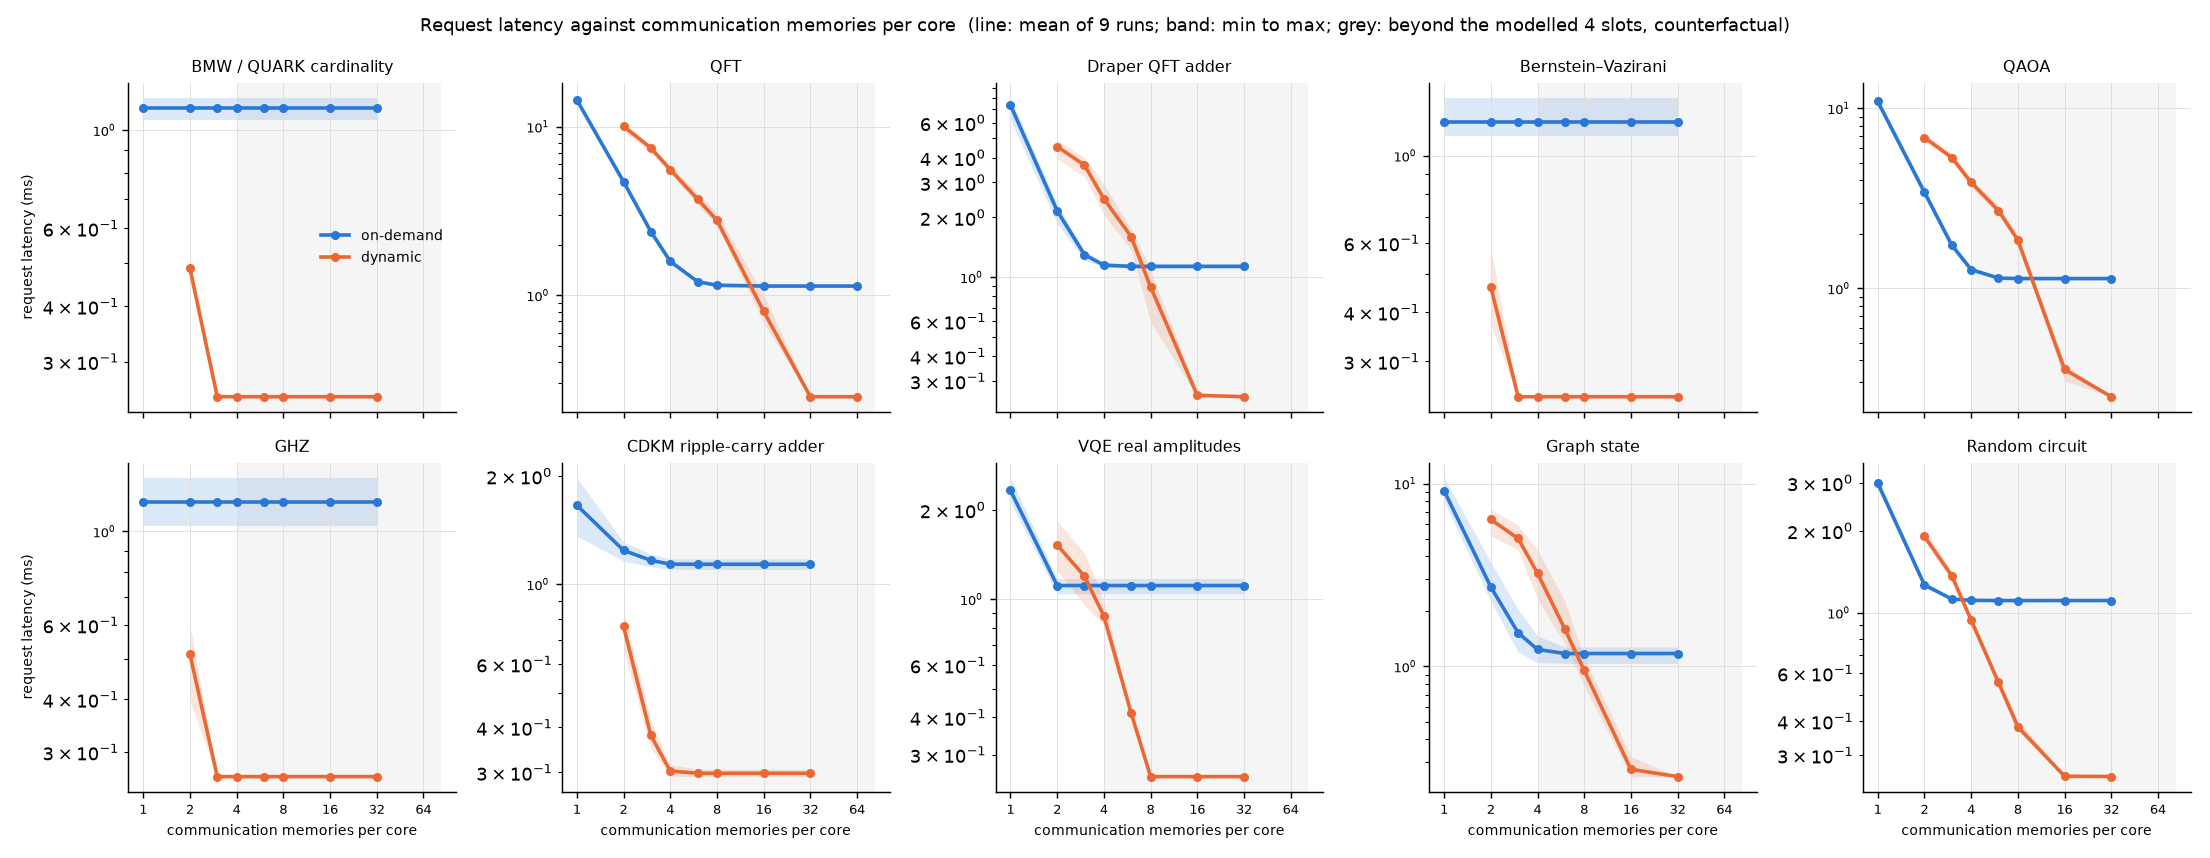
\includegraphics[width=\linewidth]{latency_vs_budget.png}
\caption{Request latency against communication memories per core. Line: mean of nine runs; band: minimum to maximum; grey: counterfactual budgets.}
\label{fig:exp1-latency}
\end{figure}

\begin{table}[H]
\centering\small
\resizebox{\ifdim\width>\linewidth\linewidth\else\width\fi}{!}{%
\begin{tabular}{@{}lrrrrrrrr@{}}
\toprule
Workload & 1 & 2 & 3 & 4 & 6$^*$ & 8$^*$ & 16$^*$ & 32$^*$ \\
\midrule
GHZ & 1.17$\pm$0.11 & 1.17$\pm$0.11 & 1.17$\pm$0.11 & 1.17$\pm$0.11 & 1.17$\pm$0.11 & 1.17$\pm$0.11 & 1.17$\pm$0.11 & 1.17$\pm$0.11 \\
Bernstein--Vazirani & 1.22$\pm$0.12 & 1.22$\pm$0.12 & 1.22$\pm$0.12 & 1.22$\pm$0.12 & 1.22$\pm$0.12 & 1.22$\pm$0.12 & 1.22$\pm$0.12 & 1.22$\pm$0.12 \\
BMW/QUARK cardinality & 1.12$\pm$0.04 & 1.12$\pm$0.04 & 1.12$\pm$0.04 & 1.12$\pm$0.04 & 1.12$\pm$0.04 & 1.12$\pm$0.04 & 1.12$\pm$0.04 & 1.12$\pm$0.04 \\
VQE real amplitudes & 2.32$\pm$0.14 & 1.11$\pm$0.05 & 1.11$\pm$0.05 & 1.11$\pm$0.05 & 1.11$\pm$0.05 & 1.11$\pm$0.05 & 1.11$\pm$0.05 & 1.11$\pm$0.05 \\
CDKM ripple-carry adder & 1.66$\pm$0.22 & 1.24$\pm$0.05 & 1.17$\pm$0.03 & 1.14$\pm$0.03 & 1.14$\pm$0.03 & 1.14$\pm$0.03 & 1.14$\pm$0.03 & 1.14$\pm$0.03 \\
Graph state & 9.14$\pm$1.14 & 2.72$\pm$0.54 & 1.53$\pm$0.30 & 1.24$\pm$0.13 & 1.18$\pm$0.08 & 1.18$\pm$0.08 & 1.18$\pm$0.08 & 1.18$\pm$0.08 \\
Draper QFT adder & 7.36$\pm$0.84 & 2.16$\pm$0.20 & 1.30$\pm$0.05 & 1.15$\pm$0.02 & 1.13$\pm$0.02 & 1.13$\pm$0.02 & 1.13$\pm$0.02 & 1.13$\pm$0.02 \\
QAOA & 10.92$\pm$0.41 & 3.42$\pm$0.14 & 1.74$\pm$0.06 & 1.27$\pm$0.02 & 1.14$\pm$0.01 & 1.13$\pm$0.01 & 1.13$\pm$0.01 & 1.13$\pm$0.01 \\
QFT & 14.42$\pm$0.35 & 4.72$\pm$0.14 & 2.39$\pm$0.09 & 1.59$\pm$0.05 & 1.21$\pm$0.02 & 1.15$\pm$0.02 & 1.13$\pm$0.02 & 1.13$\pm$0.02 \\
Random circuit & 2.99$\pm$0.10 & 1.27$\pm$0.02 & 1.12$\pm$0.01 & 1.11$\pm$0.01 & 1.11$\pm$0.01 & 1.11$\pm$0.01 & 1.11$\pm$0.01 & 1.11$\pm$0.01 \\
\bottomrule
\end{tabular}}
\caption{Request latency (ms), on-demand, mean $\pm$ sd over nine runs. Budgets marked $^*$ are counterfactual (beyond the modelled four slots).}
\label{tab:exp1-latency-ondemand}
\end{table}

Three workloads with no overload (GHZ, Bernstein--Vazirani, BMW) do not respond to the budget at all. At one memory the congested workloads are severe: QFT is about 12.7 times
its saturated latency, QAOA 9.6, graph state 7.8 and Draper 6.5. At the modelled four memories the penalty against 32 memories is $+40\%$ for QFT, $+12\%$ for QAOA, $+5\%$ for graph state and
$+1\%$ for Draper; the other workloads are within a percent. The floor, reached once nothing waits, is $1.11$ to $1.22$\,ms in every workload: that is generation time, not contention.

\begin{table}[H]
\centering\small
\resizebox{\ifdim\width>\linewidth\linewidth\else\width\fi}{!}{%
\begin{tabular}{@{}lrrrrrr@{}}
\toprule
Workload & 1 & 2 & 3 & 4 & 6$^*$ & 8$^*$ \\
\midrule
GHZ & +0\% & +0\% & +0\% & +0\% & +0\% & +0\% \\
Bernstein--Vazirani & +0\% & +0\% & +0\% & +0\% & +0\% & +0\% \\
BMW/QUARK cardinality & +0\% & +0\% & +0\% & +0\% & +0\% & +0\% \\
VQE real amplitudes & +109\% & +0\% & +0\% & +0\% & +0\% & +0\% \\
CDKM ripple-carry adder & +46\% & +9\% & +3\% & +0\% & +0\% & +0\% \\
Graph state & +676\% & +131\% & +30\% & +5\% & +0\% & +0\% \\
Draper QFT adder & +549\% & +90\% & +14\% & +1\% & +0\% & +0\% \\
QAOA & +863\% & +202\% & +53\% & +12\% & +1\% & -0\% \\
QFT & +1170\% & +316\% & +110\% & +40\% & +6\% & +1\% \\
Random circuit & +170\% & +14\% & +1\% & +0\% & +0\% & +0\% \\
\bottomrule
\end{tabular}}
\caption{On-demand latency relative to the same workload with 32 memories (saturated), by memories per core. $^*$ counterfactual.}
\label{tab:exp1-penalty}
\end{table}

\begin{table}[H]
\centering\small
\resizebox{\ifdim\width>\linewidth\linewidth\else\width\fi}{!}{%
\begin{tabular}{@{}lrrrrrrrrr@{}}
\toprule
Workload & OD 1 & OD 2 & OD 4 & OD 8 & OD 32 & Dyn 2 & Dyn 4 & Dyn 8 & Dyn 32 \\
\midrule
GHZ & 0.33 & 0.33 & 0.33 & 0.33 & 0.33 & 0.31 & 0.30 & 0.30 & 0.30 \\
Bernstein--Vazirani & 0.89 & 0.89 & 0.89 & 0.89 & 0.89 & 0.87 & 0.86 & 0.86 & 0.86 \\
BMW/QUARK cardinality & 6.95 & 6.95 & 6.95 & 6.95 & 6.95 & 6.86 & 6.83 & 6.83 & 6.83 \\
VQE real amplitudes & 0.74 & 0.68 & 0.68 & 0.68 & 0.68 & 0.68 & 0.63 & 0.61 & 0.61 \\
CDKM ripple-carry adder & 5.62 & 5.59 & 5.58 & 5.58 & 5.58 & 5.37 & 5.20 & 5.20 & 5.20 \\
Graph state & 0.38 & 0.26 & 0.24 & 0.24 & 0.24 & 0.32 & 0.26 & 0.23 & 0.22 \\
Draper QFT adder & 6.89 & 5.14 & 4.88 & 4.87 & 4.87 & 5.91 & 5.03 & 4.54 & 4.41 \\
QAOA & 10.69 & 6.60 & 5.48 & 5.40 & 5.40 & 8.50 & 6.62 & 5.52 & 4.74 \\
QFT & 9.11 & 5.72 & 4.66 & 4.51 & 4.51 & 7.50 & 5.75 & 4.79 & 4.05 \\
Random circuit & 59.78 & 51.50 & 50.89 & 50.89 & 50.89 & 53.58 & 47.74 & 45.05 & 44.58 \\
\bottomrule
\end{tabular}}
\caption{Makespan (simulated seconds of the whole circuit), on-demand (OD) and dynamic (Dyn), by memories per core. Mostly the fixed 5.3\,ms lead and 5\,ms empty-layer gap.}
\label{tab:exp1-makespan}
\end{table}

\begin{table}[H]
\centering\small
\resizebox{\ifdim\width>\linewidth\linewidth\else\width\fi}{!}{%
\begin{tabular}{@{}lrrrrrr@{}}
\toprule
Workload & 2 mem. seed 42 & 43 & 44 & 4 mem. seed 42 & 43 & 44 \\
\midrule
GHZ & 1.21 & 1.13 & 1.18 & 1.21 & 1.13 & 1.18 \\
Bernstein--Vazirani & 1.24 & 1.22 & 1.21 & 1.24 & 1.22 & 1.21 \\
BMW/QUARK cardinality & 1.11 & 1.13 & 1.11 & 1.11 & 1.13 & 1.11 \\
VQE real amplitudes & 1.15 & 1.11 & 1.08 & 1.15 & 1.11 & 1.08 \\
CDKM ripple-carry adder & 1.26 & 1.28 & 1.18 & 1.14 & 1.13 & 1.14 \\
Graph state & 2.42 & 2.33 & 3.41 & 1.19 & 1.16 & 1.36 \\
Draper QFT adder & 2.26 & 1.89 & 2.32 & 1.16 & 1.14 & 1.15 \\
QAOA & 3.59 & 3.39 & 3.28 & 1.28 & 1.29 & 1.25 \\
QFT & 4.60 & 4.91 & 4.66 & 1.57 & 1.65 & 1.55 \\
Random circuit & 1.28 & 1.27 & 1.24 & 1.11 & 1.11 & 1.11 \\
\bottomrule
\end{tabular}}
\caption{On-demand latency (ms) by mapping seed (mean over the three physics seeds): where there is congestion the mapping seed matters more than the physics seed; where nothing waits the physics noise dominates.}
\label{tab:exp1-mapseed}
\end{table}

The makespan is dominated by the fixed $5.3$\,ms lead and $5$\,ms empty-layer gap, so it moves much less than the request latency. Where there is congestion the spread between mapping seeds is several times the spread between physics seeds at two memories (graph state: $0.60$\,ms between the three mapping-seed means against $0.15$\,ms between physics seeds; Draper: $0.23$ against $0.02$); where nothing waits the physics noise dominates. Over the 20 workload-and-budget cells of Table~\ref{tab:exp1-mapseed} the mapping spread is the larger in 9.

\section{Congestion as waiting}
\begin{figure}[H]
\centering
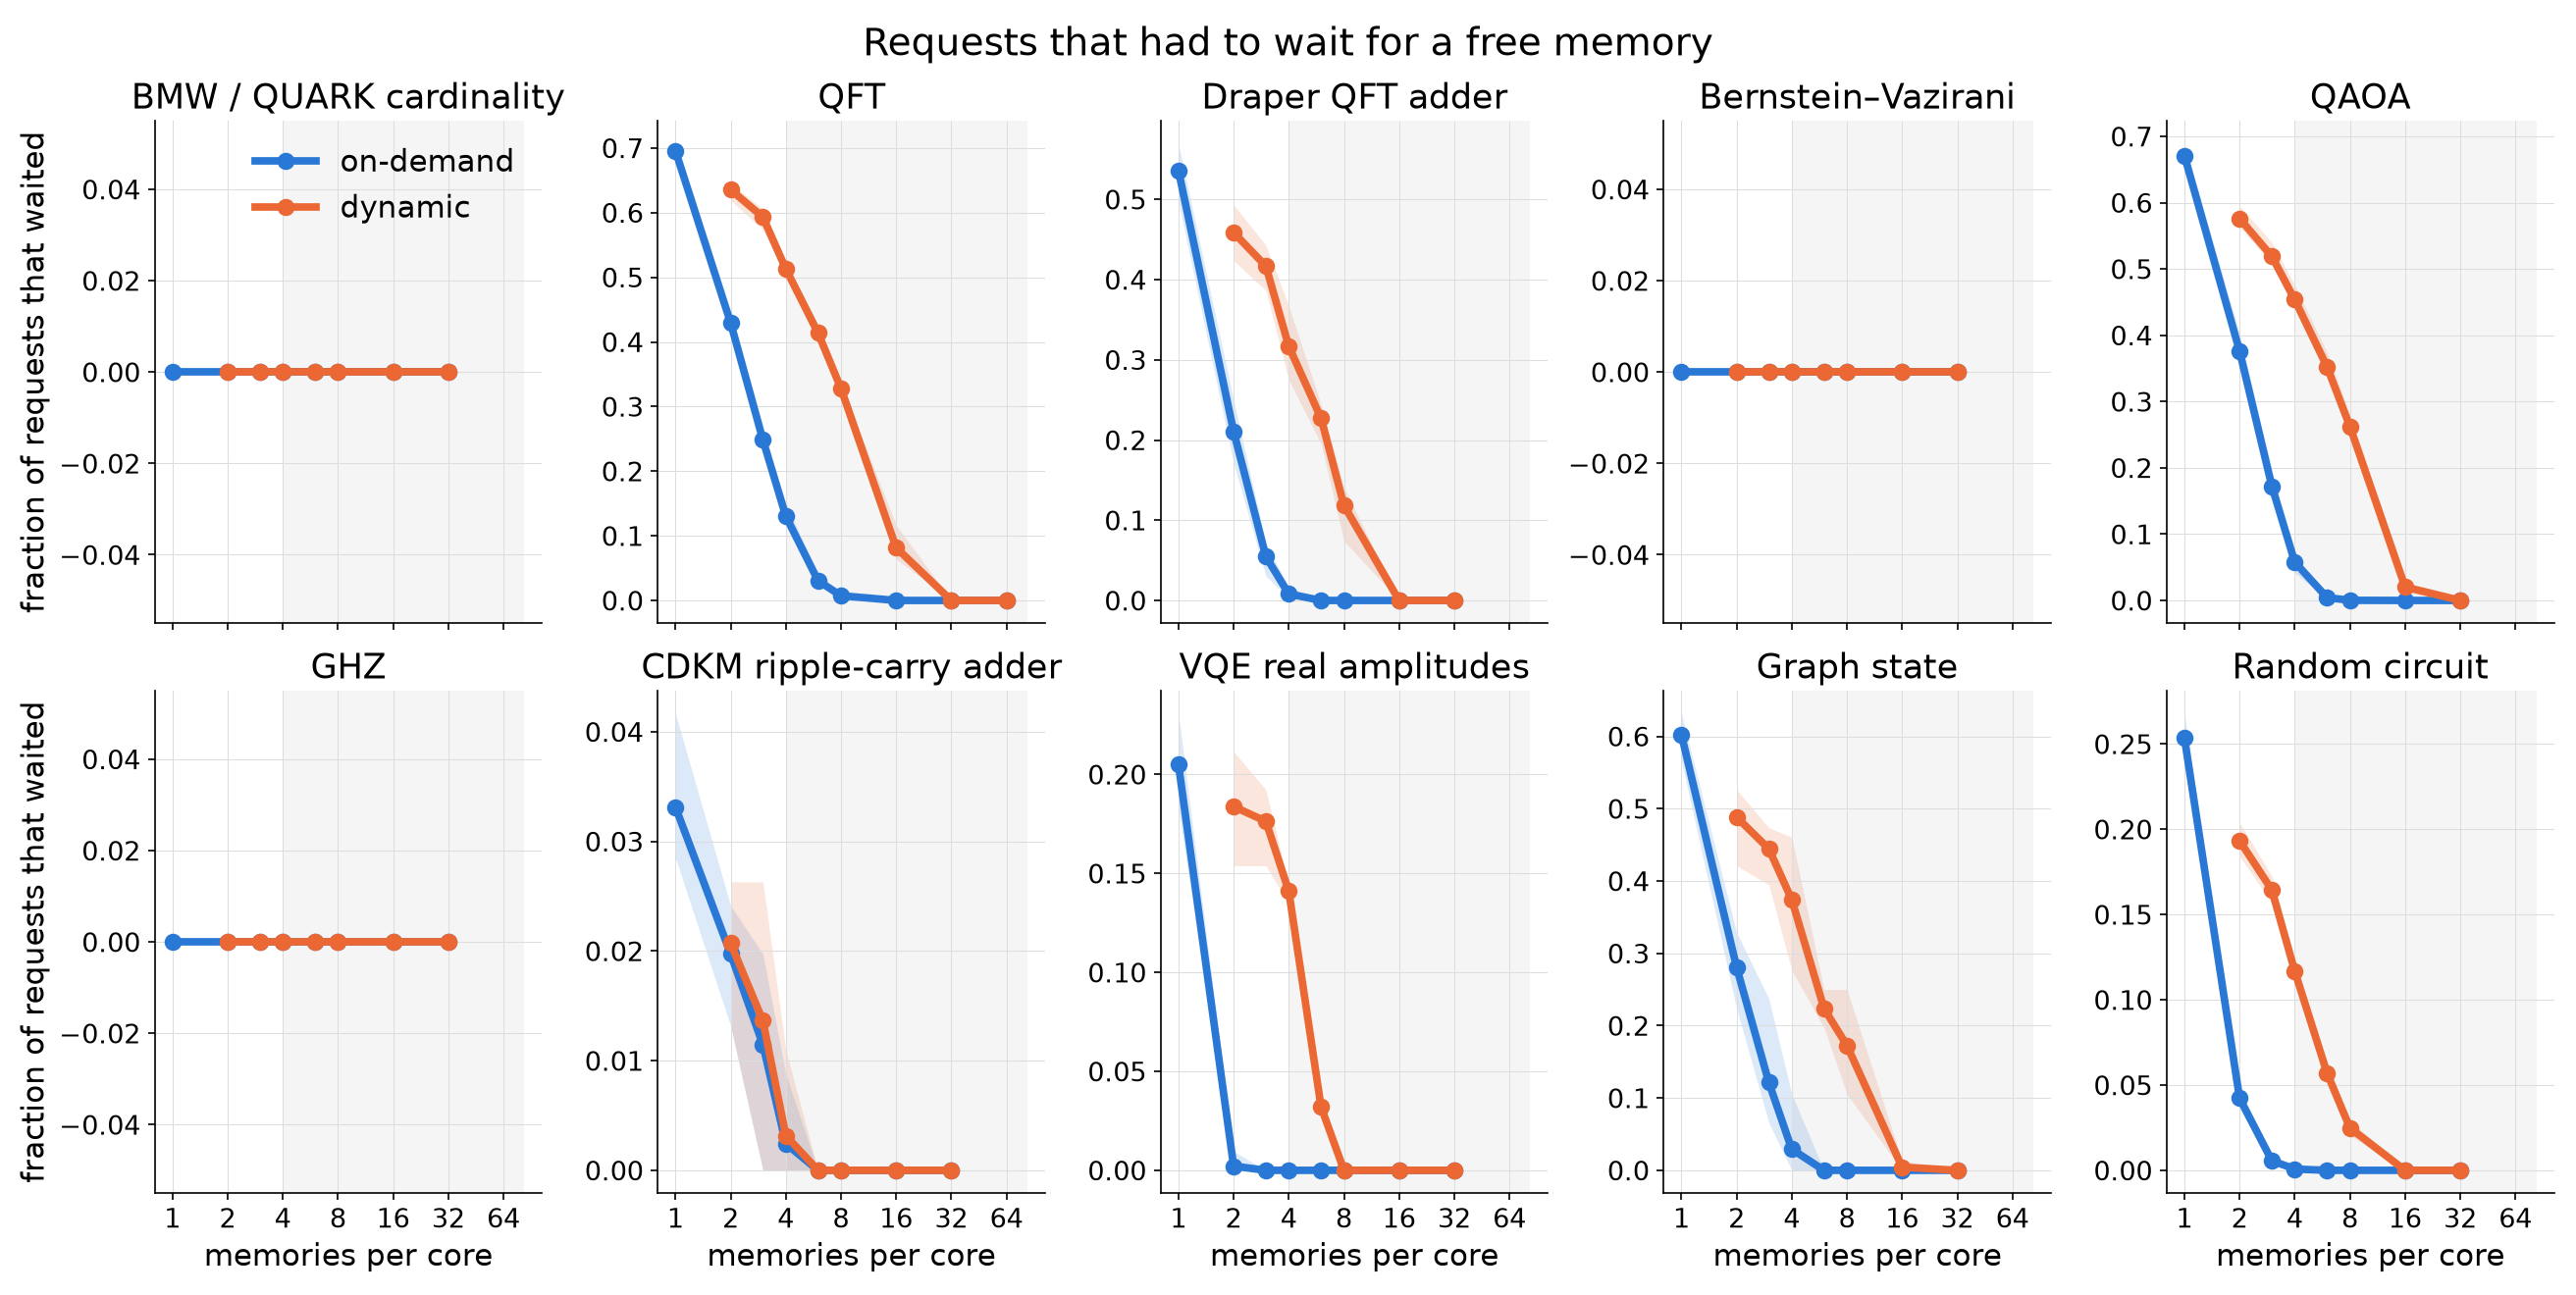
\includegraphics[width=\linewidth]{waiting_vs_budget.png}
\caption{Fraction of requests that had to wait for a free memory. Line: mean of nine runs; band: minimum to maximum; grey: counterfactual budgets.}
\label{fig:exp1-waiting}
\end{figure}

\begin{table}[H]
\centering\small
\resizebox{\ifdim\width>\linewidth\linewidth\else\width\fi}{!}{%
\begin{tabular}{@{}lrrrrrrrr@{}}
\toprule
Workload & 1 & 2 & 3 & 4 & 6$^*$ & 8$^*$ & 16$^*$ & 32$^*$ \\
\midrule
GHZ & 0.000 & 0.000 & 0.000 & 0.000 & 0.000 & 0.000 & 0.000 & 0.000 \\
Bernstein--Vazirani & 0.000 & 0.000 & 0.000 & 0.000 & 0.000 & 0.000 & 0.000 & 0.000 \\
BMW/QUARK cardinality & 0.000 & 0.000 & 0.000 & 0.000 & 0.000 & 0.000 & 0.000 & 0.000 \\
VQE real amplitudes & 0.205 & 0.002 & 0.000 & 0.000 & 0.000 & 0.000 & 0.000 & 0.000 \\
CDKM ripple-carry adder & 0.033 & 0.020 & 0.011 & 0.002 & 0.000 & 0.000 & 0.000 & 0.000 \\
Graph state & 0.602 & 0.281 & 0.121 & 0.029 & 0.000 & 0.000 & 0.000 & 0.000 \\
Draper QFT adder & 0.536 & 0.211 & 0.055 & 0.008 & 0.000 & 0.000 & 0.000 & 0.000 \\
QAOA & 0.671 & 0.376 & 0.172 & 0.058 & 0.004 & 0.000 & 0.000 & 0.000 \\
QFT & 0.696 & 0.430 & 0.249 & 0.130 & 0.031 & 0.007 & 0.000 & 0.000 \\
Random circuit & 0.254 & 0.042 & 0.006 & 0.001 & 0.000 & 0.000 & 0.000 & 0.000 \\
\bottomrule
\end{tabular}}
\caption{Fraction of requests that waited more than a microsecond for a free memory, on-demand. Budgets marked $^*$ are counterfactual (beyond the modelled four slots).}
\label{tab:exp1-waiting-ondemand}
\end{table}

\begin{table}[H]
\centering\small
\resizebox{\ifdim\width>\linewidth\linewidth\else\width\fi}{!}{%
\begin{tabular}{@{}lrrrr@{}}
\toprule
Workload & 1 memory & 2 & 3 & 4 \\
\midrule
GHZ & 20\% / +0\% & 0\% / +0\% & 0\% / +0\% & 0\% / +0\% \\
Bernstein--Vazirani & 25\% / +0\% & 0\% / +0\% & 0\% / +0\% & 0\% / +0\% \\
BMW/QUARK cardinality & 20\% / +0\% & 0\% / +0\% & 0\% / +0\% & 0\% / +0\% \\
VQE real amplitudes & 55\% / +109\% & 32\% / +0\% & 11\% / +0\% & 6\% / +0\% \\
CDKM ripple-carry adder & 96\% / +46\% & 1\% / +9\% & 1\% / +3\% & 1\% / +0\% \\
Graph state & 100\% / +676\% & 83\% / +131\% & 50\% / +30\% & 33\% / +5\% \\
Draper QFT adder & 93\% / +549\% & 65\% / +90\% & 60\% / +14\% & 41\% / +1\% \\
QAOA & 98\% / +863\% & 85\% / +202\% & 79\% / +53\% & 72\% / +12\% \\
QFT & 95\% / +1170\% & 76\% / +316\% & 76\% / +110\% & 65\% / +40\% \\
Random circuit & 90\% / +170\% & 35\% / +14\% & 25\% / +1\% & 8\% / +0\% \\
\bottomrule
\end{tabular}}
\caption{Structural overload of the traces (\% of active layers with any core above capacity) / simulated on-demand latency penalty against 32 memories, at the same capacity.}
\label{tab:exp1-struct}
\end{table}

The structural overload of the traces at the same capacity (Chapter~\ref{ch:heatmap}) predicts which workloads pay: across the 60 (workload, budget 1 to 8) points the structural overload and the
on-demand latency penalty are strongly rank-correlated (Spearman $\rho=0.85$).

\section{Pre-generation against on-demand, and the fidelity price}
\begin{table}[H]
\centering\small
\resizebox{\ifdim\width>\linewidth\linewidth\else\width\fi}{!}{%
\begin{tabular}{@{}lrrrrrrr@{}}
\toprule
Workload & 2 & 3 & 4 & 6$^*$ & 8$^*$ & 16$^*$ & 32$^*$ \\
\midrule
GHZ & 0.51$\pm$0.07 & 0.26$\pm$0.00 & 0.26$\pm$0.00 & 0.26$\pm$0.00 & 0.26$\pm$0.00 & 0.26$\pm$0.00 & 0.26$\pm$0.00 \\
Bernstein--Vazirani & 0.46$\pm$0.07 & 0.24$\pm$0.00 & 0.24$\pm$0.00 & 0.24$\pm$0.00 & 0.24$\pm$0.00 & 0.24$\pm$0.00 & 0.24$\pm$0.00 \\
BMW/QUARK cardinality & 0.49$\pm$0.02 & 0.25$\pm$0.00 & 0.25$\pm$0.00 & 0.25$\pm$0.00 & 0.25$\pm$0.00 & 0.25$\pm$0.00 & 0.25$\pm$0.00 \\
VQE real amplitudes & 1.52$\pm$0.20 & 1.19$\pm$0.16 & 0.88$\pm$0.07 & 0.41$\pm$0.00 & 0.25$\pm$0.00 & 0.25$\pm$0.00 & 0.25$\pm$0.00 \\
CDKM ripple-carry adder & 0.76$\pm$0.06 & 0.38$\pm$0.03 & 0.30$\pm$0.01 & 0.30$\pm$0.01 & 0.30$\pm$0.01 & 0.30$\pm$0.01 & 0.30$\pm$0.01 \\
Graph state & 6.36$\pm$0.79 & 5.01$\pm$0.59 & 3.23$\pm$0.82 & 1.60$\pm$0.39 & 0.95$\pm$0.13 & 0.27$\pm$0.04 & 0.25$\pm$0.00 \\
Draper QFT adder & 4.55$\pm$0.43 & 3.67$\pm$0.34 & 2.48$\pm$0.38 & 1.60$\pm$0.17 & 0.89$\pm$0.23 & 0.25$\pm$0.01 & 0.25$\pm$0.00 \\
QAOA & 6.89$\pm$0.28 & 5.33$\pm$0.19 & 3.88$\pm$0.17 & 2.70$\pm$0.13 & 1.86$\pm$0.08 & 0.35$\pm$0.04 & 0.25$\pm$0.00 \\
QFT & 10.06$\pm$0.54 & 7.49$\pm$0.33 & 5.57$\pm$0.21 & 3.73$\pm$0.25 & 2.78$\pm$0.19 & 0.80$\pm$0.16 & 0.25$\pm$0.00 \\
Random circuit & 1.91$\pm$0.08 & 1.37$\pm$0.04 & 0.94$\pm$0.02 & 0.56$\pm$0.02 & 0.38$\pm$0.02 & 0.25$\pm$0.00 & 0.25$\pm$0.00 \\
\bottomrule
\end{tabular}}
\caption{Request latency (ms), dynamic pre-generation. Budgets marked $^*$ are counterfactual (beyond the modelled four slots).}
\label{tab:exp1-latency-dynamic}
\end{table}

\begin{figure}[H]
\centering
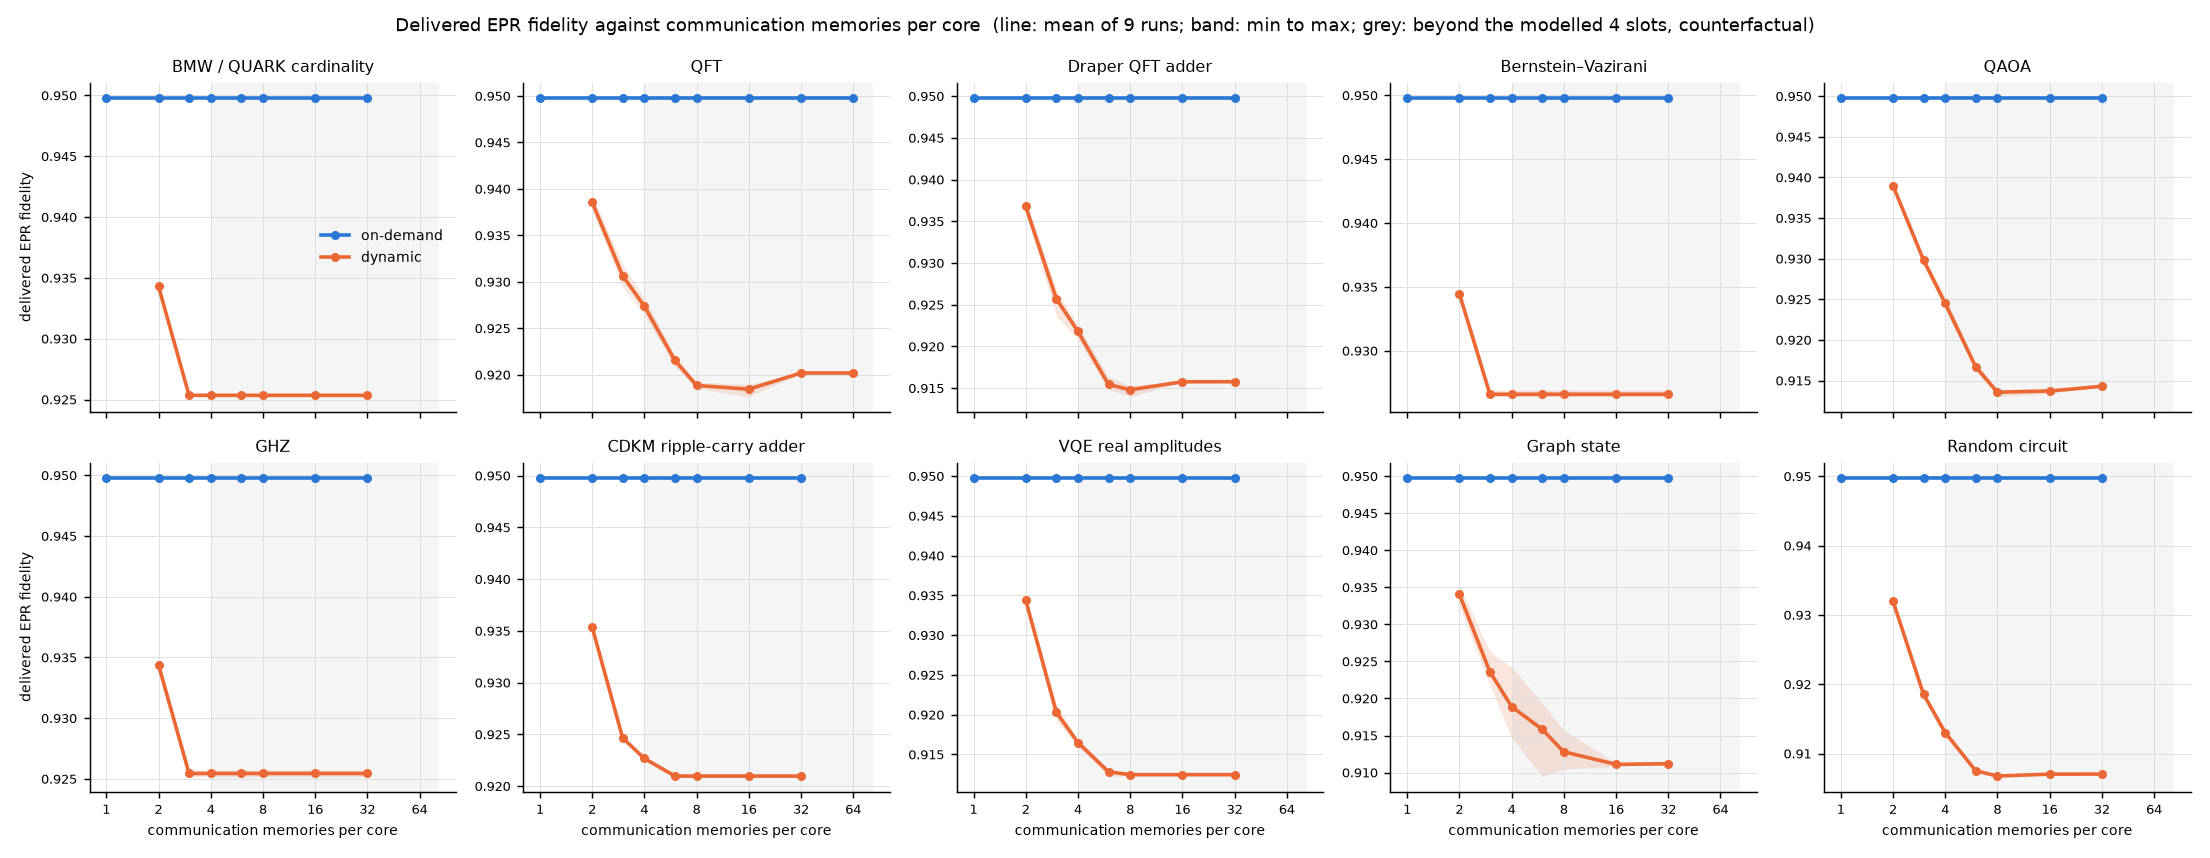
\includegraphics[width=\linewidth]{fidelity_vs_budget.png}
\caption{Delivered EPR fidelity against communication memories per core. Line: mean of nine runs; band: minimum to maximum; grey: counterfactual budgets.}
\label{fig:exp1-fidelity}
\end{figure}

\begin{table}[H]
\centering\small
\resizebox{\ifdim\width>\linewidth\linewidth\else\width\fi}{!}{%
\begin{tabular}{@{}lrrrrrrr@{}}
\toprule
Workload & 2 & 3 & 4 & 6$^*$ & 8$^*$ & 16$^*$ & 32$^*$ \\
\midrule
GHZ & 0.9344 & 0.9254 & 0.9254 & 0.9254 & 0.9254 & 0.9254 & 0.9254 \\
Bernstein--Vazirani & 0.9345 & 0.9266 & 0.9266 & 0.9266 & 0.9266 & 0.9266 & 0.9266 \\
BMW/QUARK cardinality & 0.9343 & 0.9253 & 0.9253 & 0.9253 & 0.9253 & 0.9253 & 0.9253 \\
VQE real amplitudes & 0.9344 & 0.9203 & 0.9165 & 0.9128 & 0.9125 & 0.9125 & 0.9125 \\
CDKM ripple-carry adder & 0.9354 & 0.9247 & 0.9227 & 0.9210 & 0.9210 & 0.9210 & 0.9210 \\
Graph state & 0.9341 & 0.9236 & 0.9189 & 0.9158 & 0.9128 & 0.9111 & 0.9112 \\
Draper QFT adder & 0.9368 & 0.9257 & 0.9218 & 0.9154 & 0.9148 & 0.9158 & 0.9158 \\
QAOA & 0.9390 & 0.9298 & 0.9245 & 0.9167 & 0.9136 & 0.9137 & 0.9143 \\
QFT & 0.9386 & 0.9306 & 0.9274 & 0.9215 & 0.9189 & 0.9185 & 0.9202 \\
Random circuit & 0.9320 & 0.9186 & 0.9130 & 0.9075 & 0.9068 & 0.9070 & 0.9071 \\
\bottomrule
\end{tabular}}
\caption{Delivered EPR fidelity, dynamic pre-generation. Budgets marked $^*$ are counterfactual (beyond the modelled four slots).}
\label{tab:exp1-fidelity-dynamic}
\end{table}

For the congested workloads dynamic is slower than on-demand at small budgets, because its prepared pairs may occupy up to $\text{budget}-1$ of the memories and requests then wait for a free one (Chapter~\ref{ch:why-dynamic}); the first budget at which
dynamic is faster than on-demand is 8 for graph state and Draper and 16 for QAOA and QFT. At 32 memories dynamic reaches $0.24$ to $0.30$\,ms against $1.11$ to $1.22$\,ms on-demand. Delivered fidelity under
dynamic is below the on-demand value ($0.9498$ in every cell) and falls as the compiler bank grows from two to about eight memories, by at most $0.043$ under ACE's one-second coherence time; the mechanism (pairs stored longer) is likely but was not measured.

\section{Sensitivity to the physical parameters}
This is exploratory, not a result of the study: the parameters are undecided. Five workloads, budgets $2,4,8,32$, mapping seed 42, were rerun with the group's multi-core paper's coherence time ($1$\,ms) and memory efficiency ($0.85$) in place of ACE's
($1$\,s and $0.95$). With the paper's values \textbf{every cached pair expires unused} (6 of 15\,700 compiler pairs were used), so dynamic pre-generation gives no benefit at all; on-demand fidelity falls from $0.9498$ to $0.7861$ in every workload and
budget, and on-demand latency rises by about $0.26$ to $0.42$\,ms. The congestion curves keep their shape. So the congestion results are structural and change little with these parameters, while the pre-generation and fidelity results depend entirely on them.

\section{Workload by workload}
Each paragraph is generated from the data: structural overload, the on-demand latency curve, the waiting at four memories, and the dynamic curve with the budget at which pre-generation first beats on-demand.
\subsection*{GHZ}
Structural overload at four slots: 0.0\% of active layers (one slot: 20\%). On-demand latency is 1.17\,ms with one memory, 1.17 with two, 1.17 with four and 1.17 with 32; it is within 5\% of the saturated value from 1 memory. At four memories 0.0\% of requests waited. Dynamic pre-generation takes 0.51\,ms with two memories, 0.26 with four and 0.26 with 32, and first beats on-demand at 2 memories; its delivered fidelity is 0.9344 at two memories and 0.9254 at 32 (on-demand: 0.9498).

\subsection*{Bernstein--Vazirani}
Structural overload at four slots: 0.0\% of active layers (one slot: 25\%). On-demand latency is 1.22\,ms with one memory, 1.22 with two, 1.22 with four and 1.22 with 32; it is within 5\% of the saturated value from 1 memory. At four memories 0.0\% of requests waited. Dynamic pre-generation takes 0.46\,ms with two memories, 0.24 with four and 0.24 with 32, and first beats on-demand at 2 memories; its delivered fidelity is 0.9345 at two memories and 0.9266 at 32 (on-demand: 0.9498).

\subsection*{BMW/QUARK cardinality}
Structural overload at four slots: 0.0\% of active layers (one slot: 20\%). On-demand latency is 1.12\,ms with one memory, 1.12 with two, 1.12 with four and 1.12 with 32; it is within 5\% of the saturated value from 1 memory. At four memories 0.0\% of requests waited. Dynamic pre-generation takes 0.49\,ms with two memories, 0.25 with four and 0.25 with 32, and first beats on-demand at 2 memories; its delivered fidelity is 0.9343 at two memories and 0.9253 at 32 (on-demand: 0.9498).

\subsection*{VQE real amplitudes}
Structural overload at four slots: 6.1\% of active layers (one slot: 55\%). On-demand latency is 2.32\,ms with one memory, 1.11 with two, 1.11 with four and 1.11 with 32; it is within 5\% of the saturated value from 2 memories. At four memories 0.0\% of requests waited. Dynamic pre-generation takes 1.52\,ms with two memories, 0.88 with four and 0.25 with 32, and first beats on-demand at 4 memories; its delivered fidelity is 0.9344 at two memories and 0.9125 at 32 (on-demand: 0.9498).

\subsection*{CDKM ripple-carry adder}
Structural overload at four slots: 0.6\% of active layers (one slot: 96\%). On-demand latency is 1.66\,ms with one memory, 1.24 with two, 1.14 with four and 1.14 with 32; it is within 5\% of the saturated value from 3 memories. At four memories 0.2\% of requests waited. Dynamic pre-generation takes 0.76\,ms with two memories, 0.30 with four and 0.30 with 32, and first beats on-demand at 2 memories; its delivered fidelity is 0.9354 at two memories and 0.9210 at 32 (on-demand: 0.9498).

\subsection*{Graph state}
Structural overload at four slots: 33.3\% of active layers (one slot: 100\%). On-demand latency is 9.14\,ms with one memory, 2.72 with two, 1.24 with four and 1.18 with 32; it is within 5\% of the saturated value from 6 memories. At four memories 2.9\% of requests waited. Dynamic pre-generation takes 6.36\,ms with two memories, 3.23 with four and 0.25 with 32, and first beats on-demand at 8 memories; its delivered fidelity is 0.9341 at two memories and 0.9112 at 32 (on-demand: 0.9498).

\subsection*{Draper QFT adder}
Structural overload at four slots: 41.3\% of active layers (one slot: 93\%). On-demand latency is 7.36\,ms with one memory, 2.16 with two, 1.15 with four and 1.13 with 32; it is within 5\% of the saturated value from 4 memories. At four memories 0.8\% of requests waited. Dynamic pre-generation takes 4.55\,ms with two memories, 2.48 with four and 0.25 with 32, and first beats on-demand at 8 memories; its delivered fidelity is 0.9368 at two memories and 0.9158 at 32 (on-demand: 0.9498).

\subsection*{QAOA}
Structural overload at four slots: 71.6\% of active layers (one slot: 98\%). On-demand latency is 10.92\,ms with one memory, 3.42 with two, 1.27 with four and 1.13 with 32; it is within 5\% of the saturated value from 6 memories. At four memories 5.8\% of requests waited. Dynamic pre-generation takes 6.89\,ms with two memories, 3.88 with four and 0.25 with 32, and first beats on-demand at 16 memories; its delivered fidelity is 0.9390 at two memories and 0.9143 at 32 (on-demand: 0.9498).

\subsection*{QFT}
Structural overload at four slots: 65.2\% of active layers (one slot: 95\%). On-demand latency is 14.42\,ms with one memory, 4.72 with two, 1.59 with four and 1.13 with 32; it is within 5\% of the saturated value from 8 memories. At four memories 13.0\% of requests waited. Dynamic pre-generation takes 10.06\,ms with two memories, 5.57 with four and 0.25 with 32, and first beats on-demand at 16 memories; its delivered fidelity is 0.9386 at two memories and 0.9202 at 32 (on-demand: 0.9498).

\subsection*{Random circuit}
Structural overload at four slots: 8.0\% of active layers (one slot: 90\%). On-demand latency is 2.99\,ms with one memory, 1.27 with two, 1.11 with four and 1.11 with 32; it is within 5\% of the saturated value from 3 memories. At four memories 0.1\% of requests waited. Dynamic pre-generation takes 1.91\,ms with two memories, 0.94 with four and 0.25 with 32, and first beats on-demand at 4 memories; its delivered fidelity is 0.9320 at two memories and 0.9071 at 32 (on-demand: 0.9498).

